\documentclass{beamer}

\usepackage{amsmath}
\usepackage{amssymb}
\usepackage{graphicx}
\usepackage{tikz}
\usepackage{pgfplots}
\usepackage{algorithm}
\usepackage{algorithmic}
\usepackage{bm}
\usepackage{url}

\newcommand{\x}{\mathbf{x}}
\newcommand{\y}{\mathbf{y}}
\newcommand{\z}{\mathbf{z}}
\newcommand{\w}{\mathbf{w}}
\newcommand{\bmu}{\boldsymbol{\mu}}
\newcommand{\bSigma}{\boldsymbol{\Sigma}}
\newcommand{\bPhi}{\boldsymbol{\Phi}}
\newcommand{\bnu}{\boldsymbol{\nu}}
\newcommand{\btheta}{\boldsymbol{\theta}}
\newcommand{\bomega}{\boldsymbol{\omega}}
\newcommand{\bpi}{\boldsymbol{\pi}}
% Custom colors
\definecolor{simclrblue}{RGB}{30, 144, 255}
\definecolor{simclrgreen}{RGB}{50, 205, 50}
\definecolor{simclrred}{RGB}{220, 20, 60}

\setbeamercolor{alert text}{fg=simclrred}
\setbeamercolor{structure}{fg=simclrblue}
% Custom colors
\definecolor{byolblue}{RGB}{0, 123, 191}
\definecolor{byolgreen}{RGB}{0, 150, 136}
\definecolor{byolorange}{RGB}{255, 152, 0}
\definecolor{byolred}{RGB}{244, 67, 54}

\setbeamercolor{alert text}{fg=byolred}
\setbeamercolor{structure}{fg=byolblue}

\title[MO433 - Unsupervised Learning]{MO433 - Unsupervised Learning \\ \textcolor{red}{Unsupervised Feature Learning with CNNs}} 
\author{Alexandre Xavier Falc{\~{a}}o}
\institute[IC-UNICAMP]{Institute of Computing - UNICAMP}
\date{afalcao@ic.unicamp.br}

\begin{document}

\begin{frame}
\titlepage
\end{frame}
\begin{frame}{Why Unsupervised Feature Learning?}
\begin{itemize}
\item Labels are expensive and time-consuming.
  \vspace{0.3cm}
\item Most real-world data is unlabeled.
  \vspace{0.3cm}
\item Manual annotation does not scale.
\end{itemize}
\vspace{0.3cm}\pause \textbf{Solution:} Learn meaningful
representations from \alert{data structure}.
\vspace{0.5cm}\pause
\begin{block}{Statement of the problem}
Transform high-dimensional input $\mathbf{x} \in \mathbb{R}^n$ into
compact, meaningful representations $\mathbf{z} \in \mathbb{R}^d$
(where $d \ll n$) using an encoder function:
$$f_\theta: \mathbb{R}^n \rightarrow \mathbb{R}^d$$.
\end{block}

\end{frame}

\begin{frame}{Agenda}
\begin{block}{\alert{Generative approaches}}
\vspace{0.3cm}
\textbf{Autoencoders}
\begin{itemize}
\item Encoder: $\mathbf{x} \rightarrow \mathbf{z}$
\item Decoder: $\mathbf{z} \rightarrow \hat{\mathbf{x}}$
\item Loss: $\|\mathbf{x} - \hat{\mathbf{x}}\|^2$
\end{itemize}
\end{block}
\vspace{0.3cm} \pause
\begin{block}{\alert{Discriminative approaches}}
\vspace{0.3cm}
\textbf{Self-supervised learning methods}
\begin{itemize}
\item Create artificial tasks from data.
\item Contrastive: SimCLR.
\item Non-contrastive: BYOL, DINO.
\end{itemize}
\end{block}
\end{frame}

\begin{frame}{Simple Autoencoder (dense layers only): Strategy}
  \begin{itemize}
  \item \textbf{Encoder} $f_\phi: \mathbb{R}^n \to \mathbb{R}^d$ (compression).
  \vspace{0.3cm}
  \item \textbf{Latent space} $\mathbf{z} \in \mathbb{R}^d$ where $d \ll n$.
  \vspace{0.3cm}
  \item \textbf{Decoder} $g_\theta: \mathbb{R}^d \to \mathbb{R}^n$ (reconstruction).
  \end{itemize}
  \vspace{0.5cm}
  Minimize BYOL loss
  \begin{align*}
    \mathcal{L}(\phi, \theta) &= \frac{1}{N} \sum_{i=1}^N \|\mathbf{x}_i - \hat{\mathbf{x}}_i\|^2\\
    \text{where } \hat{\mathbf{x}}_i &= g_\theta(f_\phi(\mathbf{x}_i)).
  \end{align*}
  \vspace{0.3cm}\pause
  \alert{\textbf{Encoder}} learns to store the most
  \emph{essential features} in the latent $\mathbf{z}$.

\end{frame}

\begin{frame}{Simple Autoencoder: Architecture overview}

  \begin{center}
    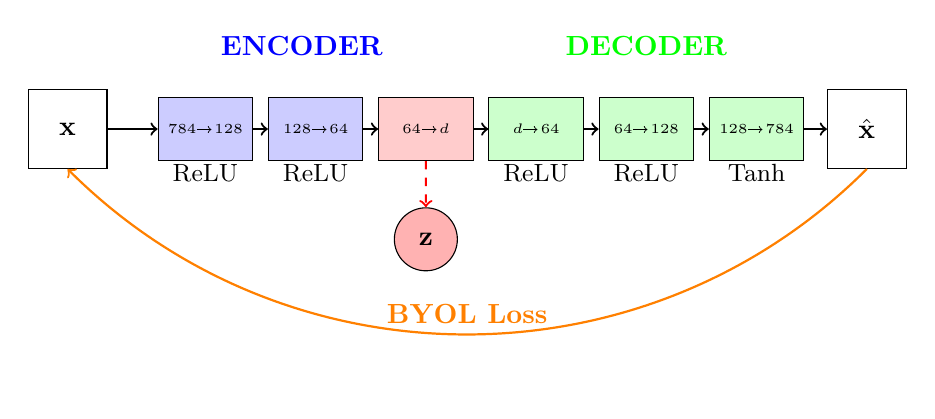
\begin{tikzpicture}[scale=0.7]
      % Input
      \node[draw, rectangle, minimum width=1.0cm, minimum height=1.0cm] (input) at (0,0) {$\mathbf{x}$};
      
      % Encoder layers
      \node[draw, rectangle, fill=blue!20, minimum width=1.2cm, minimum height=0.8cm] (enc1) at (2.5,0) {{\tiny 784→128}};
      \node[draw, rectangle, fill=blue!20, minimum width=1.2cm, minimum height=0.8cm] (enc2) at (4.5,0) {{\tiny 128→64}};
      \node[draw, rectangle, fill=red!20, minimum width=1.2cm, minimum height=0.8cm] (latent) at (6.5,0) {{\tiny 64→$d$}};
      
      % Decoder layers
      \node[draw, rectangle, fill=green!20, minimum width=1.2cm, minimum height=0.8cm] (dec1) at (8.5,0) {{\tiny $d$→64}};
     \node[draw, rectangle, fill=green!20, minimum width=1.2cm, minimum height=0.8cm] (dec2) at (10.5,0) {{\tiny 64→128}};
     \node[draw, rectangle, fill=green!20, minimum width=1.2cm, minimum height=0.8cm] (dec3) at (12.5,0) {{\tiny 128→784}};
      
      % Output
      \node[draw, rectangle, minimum width=1.0cm, minimum height=1.0cm] (output) at (14.5,0) {$\hat{\mathbf{x}}$};
      
      % Latent space
      \node[draw, circle, minimum width=0.8cm, fill=red!30] (z) at (6.5,-2) {$\mathbf{z}$};
      
      % Arrows
      \draw[->, thick] (input) -- (enc1);
      \draw[->, thick] (enc1) -- (enc2);
      \draw[->, thick] (enc2) -- (latent);
      \draw[->, thick] (latent) -- (dec1);
      \draw[->, thick] (dec1) -- (dec2);
      \draw[->, thick] (dec2) -- (dec3);
      \draw[->, thick] (dec3) -- (output);
      
      % Latent space connection
      \draw[->, thick, dashed, red] (latent) -- (z);
      
      % Labels
      \node at (4.25, 1.5) {\textcolor{blue}{\textbf{ENCODER}}};
      \node at (10.5, 1.5) {\textcolor{green}{\textbf{DECODER}}};
      
      % Reconstruction loss
     \draw[->, thick, orange, bend left=45] (output.south) to node[midway, above] {\textcolor{orange}{\textbf{BYOL Loss}}} (input.south);
      
      % ReLU activations
      \node at (2.5, -0.8) {\small ReLU};
      \node at (4.5, -0.8) {\small ReLU};
      \node at (8.5, -0.8) {\small ReLU};
      \node at (10.5, -0.8) {\small ReLU};
      \node at (12.5, -0.8) {\small Tanh};

    \end{tikzpicture}
  \end{center}
  
  \vspace{0.3cm} \textbf{Bottleneck design:} Input dimension (784) →
  Latent dimension ($d$) → Output dimension (784). The latent space
  $\mathbf{z}$ contains compressed representations.

\end{frame}


\begin{frame}{Simple Autoencoder: Reconstruction}
Even with very low latent dimension (e.g., $d=3$), the network can
produce reasonable results (code1-simple\_autoencoder.py).
\vspace{0.5cm}
  \begin{center}
    \includegraphics<1>[scale=0.7]{./figs/simple_autoencoder_1.png}
    \includegraphics<2>[scale=0.7]{./figs/simple_autoencoder_2.png}
    \includegraphics<3>[scale=0.7]{./figs/simple_autoencoder_3.png}
  \end{center}  
\end{frame}


\begin{frame}{Simple Autoencoder: Problems}
  However, it presents the following problems: 
  \vspace{0.5cm}
  \begin{itemize}
    \item By flattening images to vectors, it destroys neighborhood
      relationships.
      \vspace{0.7cm}
    \item It suffers from parameter explosion: $224 \times 224 \times 3 = 150{,}528$ inputs $\rightarrow$ millions of parameters in dense layers.
      \vspace{0.7cm}
    \item Same object at different positions $\neq$ similar encoding.
  \end{itemize}
  \vspace{0.5cm}\pause
  \alert{Convolutional autoencoders can address those problems.}
\end{frame}

\begin{frame}{Convolutional Autoencoder: Strategy}
  \begin{itemize}
  \item Addresses limitations of simple autoencoders by using \textbf{convolutional layers} 
    to preserve spatial relationships in images.
    \vspace{0.3cm}
  \item \textbf{Encoder}: Convolutions + pooling progressively reduce spatial dimensions 
    while extracting hierarchical features.
    \vspace{0.3cm}
  \item \textbf{Decoder}: Transpose convolutions + upsampling restore spatial dimensions
    from compressed feature maps.
    \vspace{0.3cm}
  \item Learns \alert{translation-invariant} features through shared convolutional filters.
    \vspace{0.3cm}
  \item Dramatically reduces parameters compared to dense layers for image data.
  \end{itemize}
\end{frame}

\begin{frame}{Convolutional Autoencoder: Strategy}
  \begin{itemize}
  \item \textbf{Encoder} $f_\phi$: Transforms input $\mathbf{x}\in \mathbb{R}^{h\times w\times c}$ into a latent $\mathbf{z}\in \mathbb{R}^{h'\times w'\times c'}$, $h' < h$, $w' < w$, $c' > c$. 
    \vspace{0.3cm}
  \item \textbf{Latent space} $\mathbf{z} \in \mathbb{R}^{h' \times w' \times c'}$ preserves spatial structure.
    \vspace{0.3cm}
  \item \textbf{Decoder} $g_\theta$: Transforms $\mathbf{z} \in \mathbb{R}^{h' \times w' \times c'}$ into $\hat{\mathbf{x}}\in \mathbb{R}^{h\times w\times c}$. 
  \end{itemize}
  \vspace{0.3cm}
  Minimize pixel-wise reconstruction loss
  \begin{align*}
    \mathcal{L}(\phi, \theta) &= \frac{1}{N} \sum_{i=1}^N \|\mathbf{x}_i - \hat{\mathbf{x}}_i\|_F^2\\
    \text{where } \hat{\mathbf{x}}_i &= g_\theta(f_\phi(\mathbf{x}_i)).
  \end{align*}

  \vspace{0.3cm}\pause
  \alert{\textbf{Encoder}} learns local patterns at multiple scales while preserving spatial relationships $\Rightarrow$ meaningful latent representations.
\end{frame}

\begin{frame}{Conv vs Simple Autoencoder: Key differences}
\begin{center}
{\tiny
  \begin{tabular}{|l|c|c|}
\hline
\textbf{Aspect} & \textbf{Simple Autoencoder} & \textbf{Conv Autoencoder} \\
\hline
\alert{Input processing} & Flatten to 784D vector & Keep 28×28×1 structure \\
\hline
\alert{Feature extraction} & Dense layers & Convolutional layers \\
\hline
\alert{Spatial awareness} & Lost after flattening & Preserved throughout \\
\hline
\alert{Translation invariance} & None & Built-in via convolutions \\
\hline
\alert{Parameter count} & Millions for large images & Much fewer (shared filters) \\
\hline
\alert{Latent representation} & 1D vector & 3D feature maps \\
\hline
  \end{tabular}
}
\end{center}

\vspace{0.5cm}\pause
\begin{alertblock}{\alert{Convolutional advantages}}
\begin{itemize}
\item \textbf{Spatial structure:} 2D relationships preserved in feature maps.
\vspace{0.3cm}
\item \textbf{Hierarchical learning:} Early layers detect edges, later layers detect objects.
\vspace{0.3cm}
\item \textbf{Efficiency:} Shared convolution kernels dramatically reduce parameters.
\end{itemize}
\end{alertblock}
\end{frame}


\begin{frame}{Convolutional Autoencoder: Architecture overview}
\begin{center}
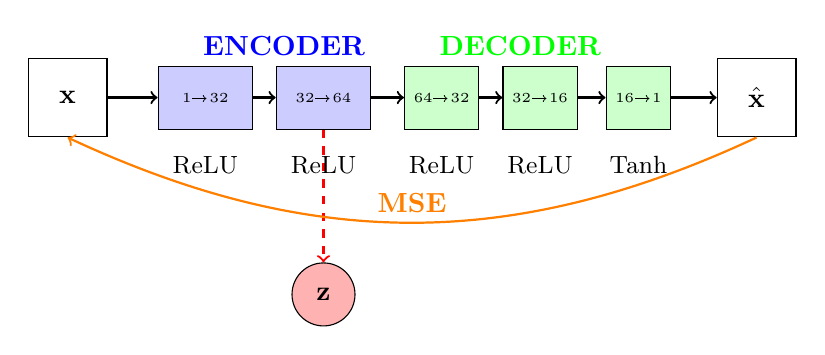
\begin{tikzpicture}[scale=0.5]
% Input
\node[draw, rectangle, minimum width=1cm, minimum height=1cm] (input) at (0,0) {$\mathbf{x}$};

% Encoder layers  
\node[draw, rectangle, fill=blue!20, minimum width=1.2cm, minimum height=0.8cm] (enc1) at (3.5,0) {\tiny 1→32};
\node[draw, rectangle, fill=blue!20, minimum width=1.2cm, minimum height=0.8cm] (enc2) at (6.5,0) {\tiny 32→64};

% Latent space (feature maps)
\node[draw, circle, fill=red!30, minimum width=0.8cm] (z) at (6.5,-5) {\textbf{z}};
      
% Decoder layers
\node[draw, rectangle, fill=green!20, minimum width=0.8cm, minimum height=0.8cm] (dec1) at (9.5,0) {\tiny 64→32};
\node[draw, rectangle, fill=green!20, minimum width=0.8cm, minimum height=0.8cm] (dec2) at (12.0,0) {\tiny 32→16};
\node[draw, rectangle, fill=green!20, minimum width=0.8cm, minimum height=0.8cm] (dec3) at (14.5,0) {\tiny 16→1};

% Output
\node[draw, rectangle, minimum width=1cm, minimum height=1cm] (output) at (17.5,0) {$\hat{\mathbf{x}}$};

% Arrows
\draw[->, thick] (input) -- (enc1);
\draw[->, thick] (enc1) -- (enc2);
\draw[->, thick] (enc2) -- (dec1);
\draw[->, thick] (dec1) -- (dec2);
\draw[->, thick] (dec2) -- (dec3);
\draw[->, thick] (dec3) -- (output);

% Latent space connection
\draw[->, thick, dashed, red] (enc2) -- (z);

% Section labels
\node at (5.5, 1.3) {\textcolor{blue}{\textbf{ENCODER}}};
\node at (11.5, 1.3) {\textcolor{green}{\textbf{DECODER}}};

% Reconstruction loss arrow
\draw[->, thick, orange, bend left=25] (output.south) to node[midway, above] {\textcolor{orange}{\textbf{MSE}}} (input.south);

% Activation labels
\node at (3.5, -1.7) {\small ReLU};
\node at (6.5, -1.7) {\small ReLU};
\node at (9.5, -1.7) {\small ReLU};
\node at (12.0, -1.7) {\small ReLU};
\node at (14.5, -1.7) {\small Tanh};

\end{tikzpicture}
\end{center}

\vspace{0.3cm} \textbf{Spatial preservation:} Input $\mathbf{x}$,
output $\hat{\mathbf{x}}$, and feature maps maintain 2D
structure. Latent space $\mathbf{z}$ ($64 \times 2 \times 2$) contains
spatial feature maps, not flattened vectors.
\end{frame}


\begin{frame}{Conv Autoencoder (code2-conv\_autoencoder.py)}
For this simple problem, both autoencoders can create accurate predictions
and improve data representation, depending on the latent dimension.
  \begin{center}
    \includegraphics<1>[scale=0.5]{./figs/conv_autoencoder_1.png}
    \includegraphics<2>[scale=0.5]{./figs/conv_autoencoder_2.png}
    \includegraphics<3>[scale=0.5]{./figs/conv_autoencoder_3.png}
    \includegraphics<4>[scale=0.6]{./figs/umap_autoencoders.pdf}
  \end{center}
  
  \vspace{0.3cm} \onslide<4>{ While autoencoders learn useful
    representations through reconstruction, \textbf{can discriminative
      approaches do better?}  }
\end{frame}

\begin{frame}{Self-supervised learning}
  \begin{itemize}
    \item Creating a \alert{pretext task} from unlabeled data enables
      learning meaningful data representations without manual
      annotations.
\vspace{0.3cm}
\item The resulting encoder can then \alert{transfer knowledge} to
  solve downstream \alert{target tasks}.
\vspace{0.3cm}
\item The network solving the target task requires \alert{considerably
  less} labeled data for training.
  \end{itemize}
  \begin{center}
    \includegraphics<1>[scale=0.30]{./figs/selfsup-learning-a.pdf}
    \includegraphics<2>[scale=0.25]{./figs/selfsup-learning-b.pdf}
    \end{center}
\end{frame}

\begin{frame}{Self-supervised learning}
  The pretext tasks became more abstract (e.g., maximize agreement
  between augmented views) after 2020:
    \vspace{0.5cm}
  \begin{itemize}
  \item SimCLR: Simple Framework for Contrastive Learning of Visual Representations [3].
    \vspace{0.5cm}
  \item BYOL: Bootstrap Your Own Latent [4].
    \vspace{0.5cm}
  \item DINO: Self-Distillation with No Labels [5].
  \end{itemize}
  \vspace{0.5cm}\pause

  \alert{Focus is shifted to learning good general representations
    rather than solving auxiliary tasks.}
\end{frame}

\begin{frame}{SimCLR: Strategy}
  
\begin{itemize}
\item The method trains an \textbf{encoder} followed by a \textbf{projector}
by \textbf{contrastive learning}. 
\vspace{0.5cm}
\item It creates \textbf{augmented pairs} from unlabeled images and
  learns to distinguish between similar and dissimilar pairs by using
  a contrastive loss.
\vspace{0.5cm}
\item Representations of augmented versions of a same image should be
  \alert{similar}, while different images should have
  \alert{dissimilar} representations.
\end{itemize}
\end{frame}

\begin{frame}{SimCLR: Architecture overview}
\begin{center}
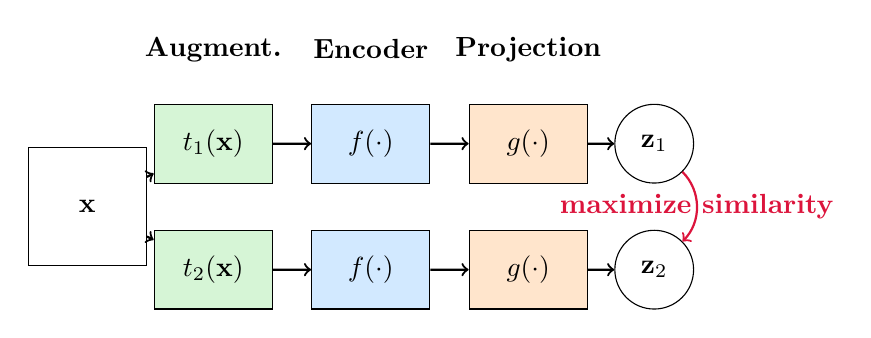
\begin{tikzpicture}[scale=0.8]
% Input image
\node[draw, rectangle, minimum width=1.5cm, minimum height=1.5cm] (input) at (0,0) {$\mathbf{x}$};

% Augmentations
\node[draw, rectangle, fill=simclrgreen!20, minimum width=1.5cm, minimum height=1cm] (aug1) at (2,1) {$t_1(\mathbf{x})$};
\node[draw, rectangle, fill=simclrgreen!20, minimum width=1.5cm, minimum height=1cm] (aug2) at (2,-1) {$t_2(\mathbf{x})$};

% Encoder
\node[draw, rectangle, fill=simclrblue!20, minimum width=1.5cm, minimum height=1cm] (enc1) at (4.5,1) {$f(\cdot)$};
\node[draw, rectangle, fill=simclrblue!20, minimum width=1.5cm, minimum height=1cm] (enc2) at (4.5,-1) {$f(\cdot)$};

% Projection head
\node[draw, rectangle, fill=orange!20, minimum width=1.5cm, minimum height=1cm] (proj1) at (7,1) {$g(\cdot)$};
\node[draw, rectangle, fill=orange!20, minimum width=1.5cm, minimum height=1cm] (proj2) at (7,-1) {$g(\cdot)$};

% Output representations
\node[draw, circle, minimum width=1cm] (z1) at (9,1) {$\mathbf{z}_1$};
\node[draw, circle, minimum width=1cm] (z2) at (9,-1) {$\mathbf{z}_2$};

% Arrows
\draw[->, thick] (input) -- (aug1);
\draw[->, thick] (input) -- (aug2);
\draw[->, thick] (aug1) -- (enc1);
\draw[->, thick] (aug2) -- (enc2);
\draw[->, thick] (enc1) -- (proj1);
\draw[->, thick] (enc2) -- (proj2);
\draw[->, thick] (proj1) -- (z1);
\draw[->, thick] (proj2) -- (z2);

% Labels
\node at (2, 2.5) {\textbf{Augment.}};
\node at (4.5, 2.5) {\textbf{Encoder}};
\node at (7, 2.5) {\textbf{Projection}};

% Similarity arrow
\draw[->, thick, simclrred, bend left=45] (z1) to node[midway, midway] {\textcolor{simclrred}{\textbf{maximize similarity}}} (z2);
\end{tikzpicture}
\end{center}
\vspace{0.5cm}
\textbf{Shared weights:} Both augmented views use the same encoder $f$ and projection head $g$.
\end{frame}

\begin{frame}{SimCLR: Data augmentation}
  \alert{Diverse views} of the same image are created through random
  transformations.
\vspace{0.3cm}
\begin{itemize}
\item \texttt{RandomRotation(20°)} - Rotational invariance.
\vspace{0.3cm}
\item \texttt{RandomAffine} with translation (±10\%) and scaling (0.9-1.1×).
\vspace{0.3cm}
\item \texttt{RandomHorizontalFlip} - Spatial invariance.  
\vspace{0.3cm}
\item \texttt{Gaussian noise} addition - Robustness to noise.
\end{itemize}
\vspace{0.5cm}
\begin{alertblock}{Critical insight.}
Strong augmentation is \alert{essential} for SimCLR success. Weak
augmentations lead to trivial solutions where the model learns
shortcuts rather than meaningful representations.
\end{alertblock}
\end{frame}

\begin{frame}{SimCLR: Data augmentation}
  Example of data augmentations.
  \vspace{0.3cm}
  \begin{center}
    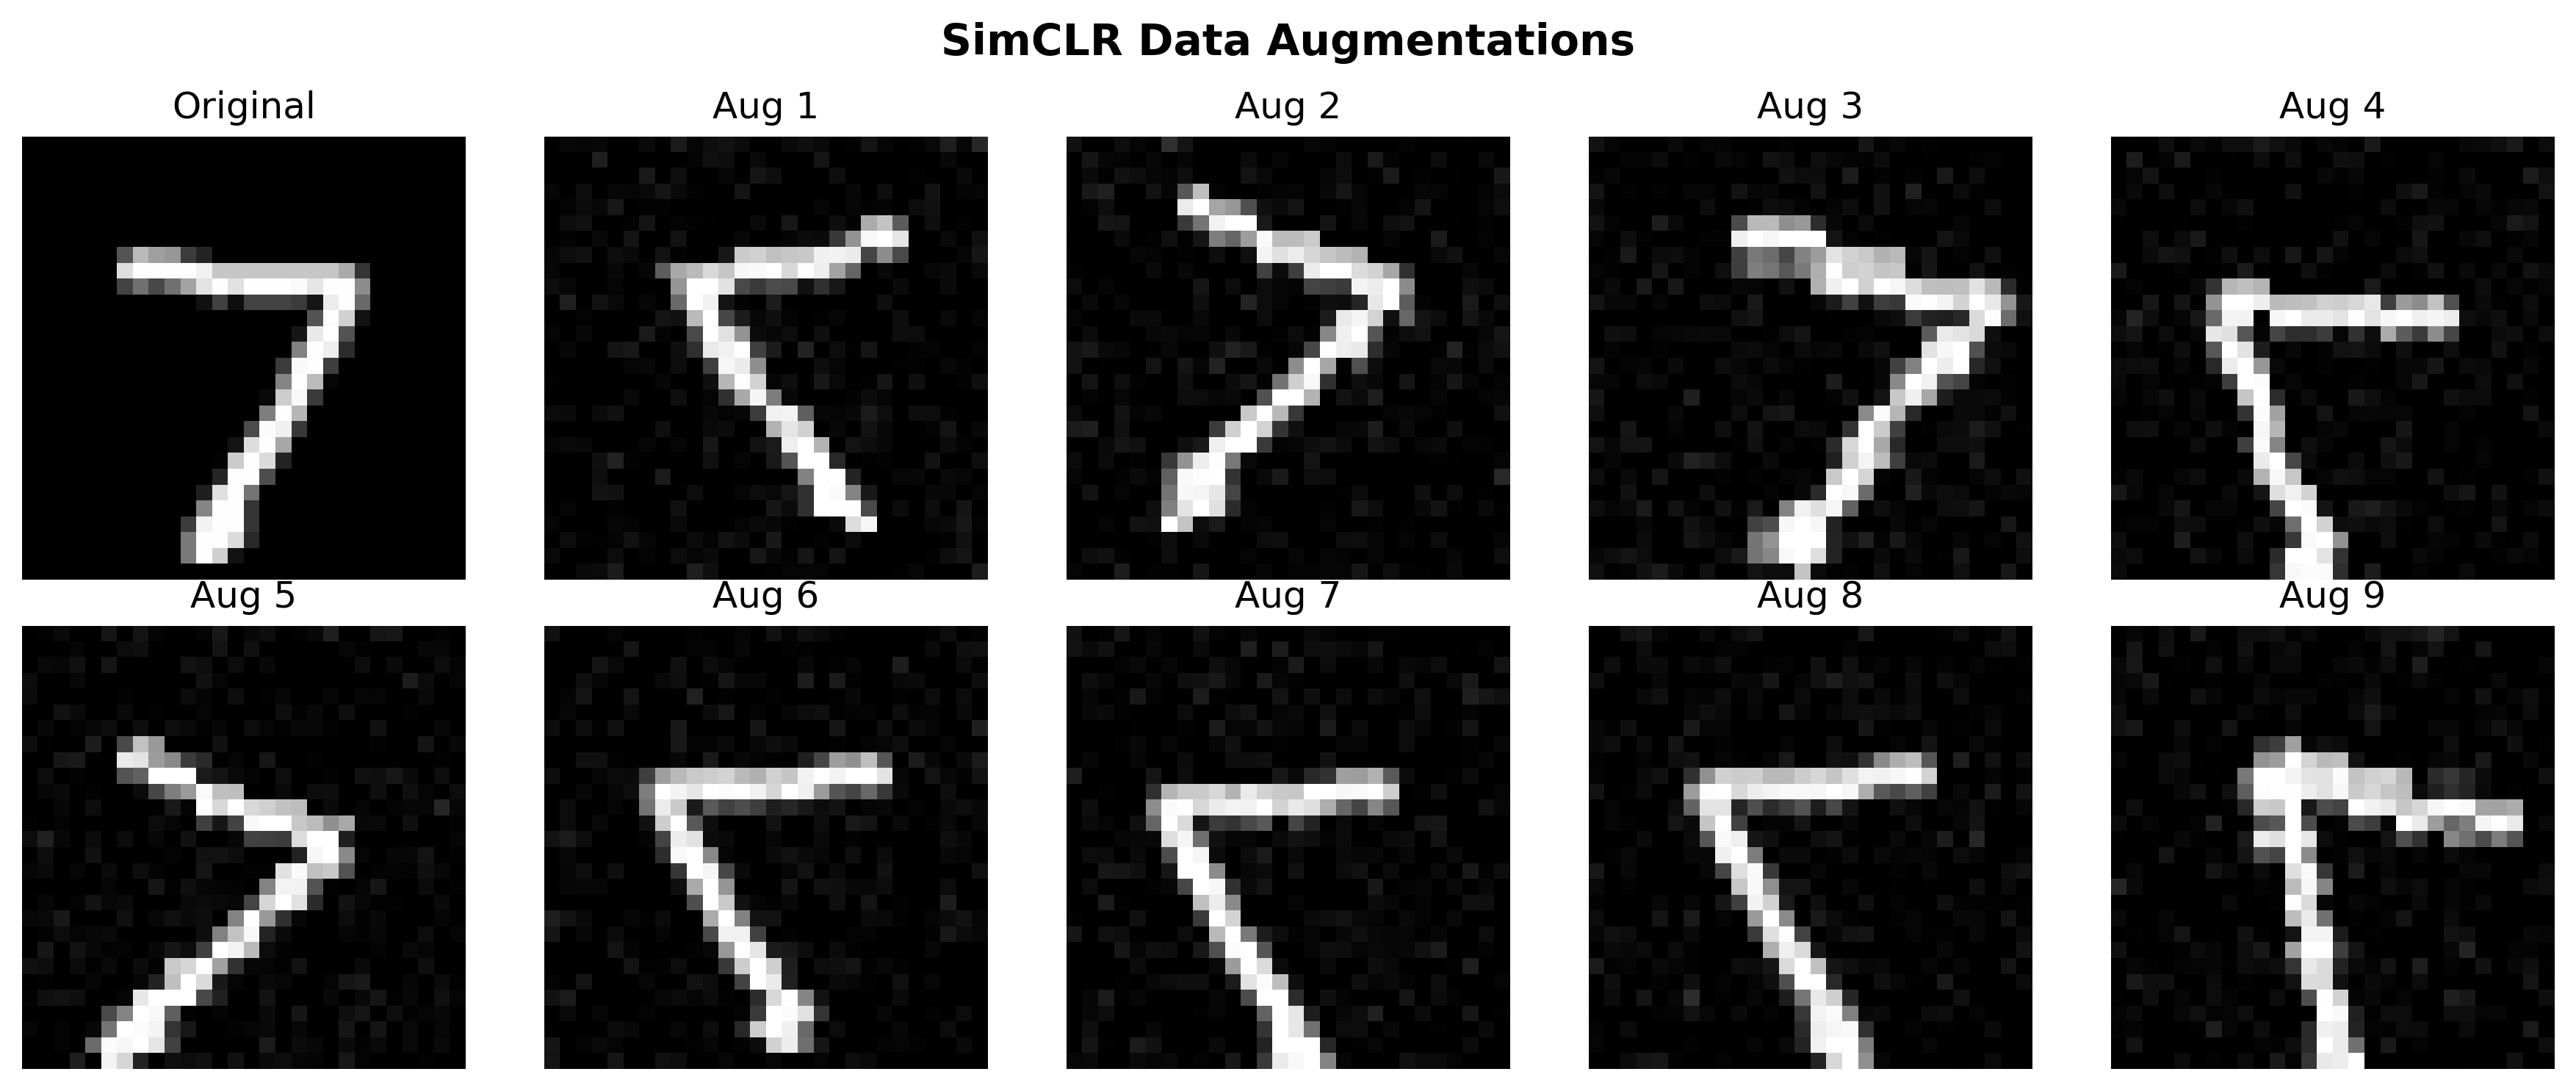
\includegraphics[scale=0.3]{./figs/simclr_augmentations.png}
  \end{center}
\end{frame}

\begin{frame}{SimCLR: Encoder architecture}
\textbf{CNN-based feature extractor:}
$$\mathbf{h} = f_\theta(\mathbf{x}) \in \mathbb{R}^d$$

\vspace{0.3cm}
Implementation details for MNIST:
\begin{itemize}
\item \textbf{Convolutional layers:} Extract spatial features.
  \begin{itemize}
  \item Conv2d(1→32) + BatchNorm + ReLU + MaxPool.
  \item Conv2d(32→64) + BatchNorm + ReLU + MaxPool.
  \end{itemize}
\vspace{0.2cm}
\item \textbf{Feature dimension:} $64 \times 2 \times 2 = 256$ features.
\vspace{0.2cm}
\item \textbf{Parameter sharing:} Same encoder processes both augmented views.
\end{itemize}

\vspace{0.3cm} \textbf{Key principle:} The encoder learns to extract
features that are \alert{invariant} to the augmentations but
\alert{discriminative} between different images.
\end{frame}

\begin{frame}{SimCLR: Projection head}
\textbf{Nonlinear projection for contrastive learning}
$$\mathbf{z} = g_\phi(\mathbf{h}) = W_2 \sigma(W_1 \mathbf{h}) \in \mathbb{R}^{128}$$

\vspace{0.3cm}
\begin{itemize}
\item \textbf{Two-layer MLP:} $256 \rightarrow 256 \rightarrow 128$.
\item \textbf{ReLU activation:} Nonlinear transformation.
\item \textbf{Lower dimensionality:} Projects to contrastive learning space.
\end{itemize}

\vspace{0.5cm}
\begin{alertblock}{Why a projection head?}
\begin{itemize}
\item Contrastive learning works better in \alert{lower-dimensional} spaces.
\item Separates representation learning from contrastive optimization.
\item \textbf{Key insight:} Use $\mathbf{h}$ for downstream tasks, not $\mathbf{z}$.
\end{itemize}
\end{alertblock}
\end{frame}

\begin{frame}{SimCLR: InfoNCE loss (NT-Xent)}
\textbf{Contrastive learning objective}
For a batch of $N$ images, create $2N$ augmented views. The loss for positive pair $(i, j)$ is:
$$\ell_{i,j} = -\log \frac{\exp(\text{sim}(\mathbf{z}_i, \mathbf{z}_j) / \tau)}{\sum_{k=1}^{2N} \mathbf{1}_{k \neq i} \exp(\text{sim}(\mathbf{z}_i, \mathbf{z}_k) / \tau)}$$

\vspace{0.3cm}
where:
\begin{itemize}
\item $\text{sim}(\mathbf{z}_i, \mathbf{z}_j) = \mathbf{z}_i^T \mathbf{z}_j / (\|\mathbf{z}_i\| \|\mathbf{z}_j\|)$ (cosine similarity).
\item $\tau$ = temperature parameter (0.5 in implementation).
\item $\mathbf{1}_{k \neq i}$ excludes self-similarity.
\end{itemize}

\vspace{0.3cm}
\textbf{Intuition:} 
\begin{itemize}
\item \alert{Numerator:} Similarity to positive pair (augmented version).
\item \alert{Denominator:} Similarities to all negatives (other images).
\end{itemize}
\end{frame}

\begin{frame}{Why SimCLR works?}
\textbf{Contrastive objective interpretation}
The InfoNCE loss can be viewed as:
$$\mathcal{L} = -\mathbb{E}\left[ \log \frac{\exp(\mathbf{z}_i^T \mathbf{z}_j / \tau)}{\exp(\mathbf{z}_i^T \mathbf{z}_j / \tau) + \sum_{k \neq i,j} \exp(\mathbf{z}_i^T \mathbf{z}_k / \tau)} \right]$$
\vspace{0.2cm}
This encourages:
\begin{itemize}
\item \alert{Alignment:} Positive pairs have high cosine similarity
  $$\mathbf{z}_i^T \mathbf{z}_j \rightarrow \|\mathbf{z}_i\| \|\mathbf{z}_j\| \cos(0) = 1$$
\item \alert{Uniformity:} Features spread uniformly on unit hypersphere
  $$\mathbb{E}_{i \neq j}[\mathbf{z}_i^T \mathbf{z}_j] \rightarrow 0$$
\end{itemize}
\vspace{0.3cm}
\textbf{Result:} Learned representations capture semantic similarity while preserving discriminative power (code3-simclr\_unsupfeatlearn.py).
\end{frame}

\begin{frame}{BYOL: Strategy}
  \begin{itemize}
  \item The method trains \textbf{online} and \textbf{target} networks.
    \begin{itemize}
    \item \textbf{Online:} Encoder + Projector + \alert{Predictor}.
    \item \textbf{Target:} Encoder + Projector.
    \end{itemize}    
    \vspace{0.5cm}
  \item Two \textbf{augmented views} of the same image are passed through \alert{both networks} (4 forward passes total). 
    \vspace{0.5cm}
  \item The online  \alert{predicts} target network's representations.
    \vspace{0.5cm}
  \item While the online's parameters are updated using \alert{BYOL
    loss}, the target uses \alert{momentum} updates to prevent
    collapse by creating a \alert{moving target} that evolves slowly.
$$\theta_{\text{target}} \leftarrow \tau \theta_{\text{target}} + (1-\tau) \theta_{\text{online}}$$
  \end{itemize}
\end{frame}

\begin{frame}{BYOL vs SimCLR: Fundamental differences}
\begin{center}
{\tiny
  \begin{tabular}{|l|c|c|}
\hline
\textbf{Aspect} & \textbf{SimCLR} & \textbf{BYOL} \\
\hline
\alert{Negative samples} & Required (large batches) & Not needed \\
\hline
\alert{Loss function} & InfoNCE (contrastive) & Cosine-based \\
\hline
\alert{Architecture} & Symmetric & Asymmetric \\
\hline
\alert{Batch dependency} & Strong (more negatives = better) & Weak \\
\hline
\alert{Key mechanism} & Contrast positive/negative & Momentum target updates \\
\hline
  \end{tabular}
}
\end{center}
\textbf{BYOL may use the same data augmentation operations as SimCLR.}

\vspace{0.5cm}\pause
\begin{alertblock}{\alert{BYOL's advantages.}}
\begin{itemize}
\item \textbf{Simpler training:} No need to manage negative samples.
\vspace{0.3cm}
\item \textbf{Batch size flexibility:} Performance less sensitive to batch size.
\vspace{0.3cm}
\item \textbf{Stable training:} Momentum updates provide stability.
\end{itemize}
\end{alertblock}
\end{frame}

\begin{frame}{BYOL: Architecture overview}
\begin{center}
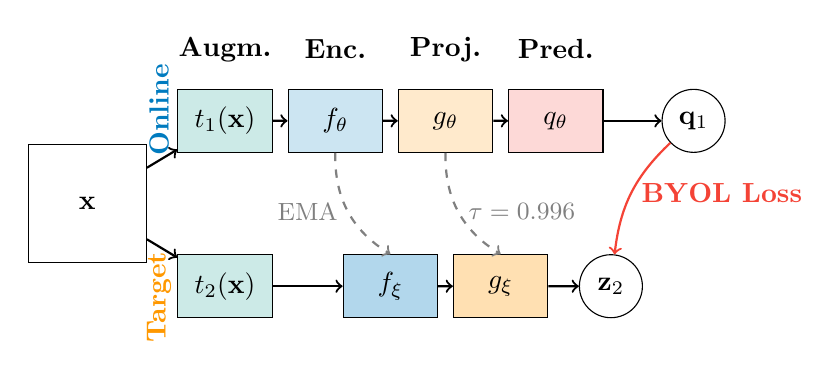
\begin{tikzpicture}[scale=0.7]
% Input image
\node[draw, rectangle, minimum width=1.5cm, minimum height=1.5cm] (input) at (0,0) {$\mathbf{x}$};

% Augmentations
\node[draw, rectangle, fill=byolgreen!20, minimum width=1.2cm, minimum height=0.8cm] (aug1) at (2.5,1.5) {$t_1(\mathbf{x})$};
\node[draw, rectangle, fill=byolgreen!20, minimum width=1.2cm, minimum height=0.8cm] (aug2) at (2.5,-1.5) {$t_2(\mathbf{x})$};

% Online network (top path)
\node[draw, rectangle, fill=byolblue!20, minimum width=1.2cm, minimum height=0.8cm] (enc_online) at (4.5,1.5) {$f_\theta$};
\node[draw, rectangle, fill=byolorange!20, minimum width=1.2cm, minimum height=0.8cm] (proj_online) at (6.5,1.5) {$g_\theta$};
\node[draw, rectangle, fill=byolred!20, minimum width=1.2cm, minimum height=0.8cm] (pred_online) at (8.5,1.5) {$q_\theta$};

% Target network (bottom path)
\node[draw, rectangle, fill=byolblue!30, minimum width=1.2cm, minimum height=0.8cm] (enc_target) at (5.5,-1.5) {$f_\xi$};
\node[draw, rectangle, fill=byolorange!30, minimum width=1.2cm, minimum height=0.8cm] (proj_target) at (7.5,-1.5) {$g_\xi$};

% Outputs
\node[draw, circle, minimum width=0.8cm] (z_online) at (11,1.5) {$\mathbf{q}_1$};
\node[draw, circle, minimum width=0.8cm] (z_target) at (9.5,-1.5) {$\mathbf{z}_2$};

% Arrows
\draw[->, thick] (input) -- (aug1);
\draw[->, thick] (input) -- (aug2);
\draw[->, thick] (aug1) -- (enc_online);
\draw[->, thick] (enc_online) -- (proj_online);
\draw[->, thick] (proj_online) -- (pred_online);
\draw[->, thick] (pred_online) -- (z_online);

\draw[->, thick] (aug2) -- (enc_target);
\draw[->, thick] (enc_target) -- (proj_target);
\draw[->, thick] (proj_target) -- (z_target);

% Loss connection
\draw[->, thick, byolred, bend right=20] (z_online) to node[midway, right] {\textcolor{byolred}{\textbf{BYOL Loss}}} (z_target);

% Labels
\node at (2.5, 2.8) {\textbf{Augm.}};
\node at (4.5, 2.8) {\textbf{Enc.}};
\node at (6.5, 2.8) {\textbf{Proj.}};
\node at (8.5, 2.8) {\textbf{Pred.}};

\node at (1.3, 1.7) [rotate=90] {\textcolor{byolblue}{\textbf{Online}}};
\node at (1.3, -1.7) [rotate=90] {\textcolor{byolorange}{\textbf{Target}}};

% Momentum update arrow
\draw[->, dashed, thick, gray] (enc_online.south) to[bend right=30] node[midway, left] {\small EMA} (enc_target.north);
\draw[->, dashed, thick, gray] (proj_online.south) to[bend right=30] node[midway, right] {\small $\tau = 0.996$} (proj_target.north);
\end{tikzpicture}
\end{center}

\vspace{0.3cm} \textbf{Key Asymmetry:} Only online network has
predictor $q_\theta$. Target network $\xi$ updated via exponential
moving average (EMA). Disable target gradients to prevent
backpropagation.
\end{frame}

\begin{frame}{BYOL: Asymmetric network design}
\textbf{Online network (trainable):}
$$\mathbf{q}_1 = q_\theta(g_\theta(f_\theta(\mathbf{x}_1)))$$
\begin{itemize}
\item \textbf{Encoder:} $f_\theta$ - extracts features.
\item \textbf{Projector:} $g_\theta$ - maps to representation space.  
\item \textbf{Predictor:} $q_\theta$ - predicts target representations.
\end{itemize}
\textbf{Target network (momentum updated):}
$$\mathbf{z}_2 = g_\xi(f_\xi(\mathbf{x}_2))$$
\begin{itemize}
\item \textbf{Encoder:} $f_\xi$ - same architecture as online.
\item \textbf{Projector:} $g_\xi$ - same architecture as online.
\item \textbf{No predictor} - key architectural difference.
\end{itemize}

\end{frame}

\begin{frame}{BYOL: Implementation}
  For MNIST:
  \textbf{Encoders:} 
  \vspace{0.3cm}
  \begin{itemize}
  \item Conv2d(1→32) + BatchNorm + ReLU + MaxPool.
    \vspace{0.3cm}
  \item Conv2d(32→64) + BatchNorm + ReLU + MaxPool.  
    \vspace{0.3cm}
  \item Feature dimension: 256 ($64 \times 2 \times 2$).
  \end{itemize}

\vspace{0.5cm}

\textbf{Projectors:} MLP(256 → 256 → 64) + BatchNorm + ReLU.

\vspace{0.5cm}

\textbf{Predictor:} MLP(64 → 32 → 64) + BatchNorm + ReLU.

\end{frame}

\begin{frame}{BYOL: Momentum update mechanism}
\textbf{Exponential Moving Average (EMA)}
Target network parameters are updated as:
$$\xi \leftarrow \tau \xi + (1 - \tau) \theta$$
where $\tau \in [0, 1]$ is the momentum coefficient.

\vspace{0.3cm}

Implementation details:
\begin{itemize}
\item \textbf{Initialization:} $\xi_0 = \theta_0$ (target = online at start).
\vspace{0.3cm}
\item \textbf{Momentum schedule:} $\tau$ increases from 0.99 to 0.999 during training.
\vspace{0.3cm}
\item \textbf{Update frequency:} Every training step (after gradient update of the online network).
\end{itemize}

\end{frame}

\begin{frame}{BYOL: Loss function}
\textbf{Symmetric cosine-based loss:}
For augmented pair $(\mathbf{x}_1, \mathbf{x}_2)$,
\begin{align*}
\mathcal{L}_{BYOL} = 2 -  \frac{\mathbf{q}_1 \cdot \mathbf{z}_2}{\|\mathbf{q}_1\| \|\mathbf{z}_2\|} -  \frac{\mathbf{q}_2 \cdot \mathbf{z}_1}{\|\mathbf{q}_2\| \|\mathbf{z}_1\|}
\end{align*}
  \vspace{0.3cm}
where:
\begin{itemize}
\item $\mathbf{q}_1 = q_\theta(g_\theta(f_\theta(\mathbf{x}_1)))$ - online prediction for view 1.
  \vspace{0.3cm}
\item $\mathbf{q}_2 = q_\theta(g_\theta(f_\theta(\mathbf{x}_2)))$ - online prediction for view 2.
  \vspace{0.3cm}
\item $\mathbf{z}_1 = g_\xi(f_\xi(\mathbf{x}_1))$ - target projection for view 1.
  \vspace{0.3cm}
\item $\mathbf{z}_2 = g_\xi(f_\xi(\mathbf{x}_2))$ - target projection for view 2.
\end{itemize}
\end{frame}

\begin{frame}{Why BYOL works?}
Without negatives, why does not the model learn trivial constant
representations (i.e., does not collapse)?
   \vspace{0.3cm}
\begin{enumerate}
\item \textbf{Asymmetric architecture:} Target has no predictor.
\vspace{0.3cm}
   \begin{itemize}
   \item Online network learns to predict target representations.
   \item Creates learning pressure without direct target optimization.
   \end{itemize}
\vspace{0.3cm}   
\item \textbf{Momentum updates:} $\xi \leftarrow \tau \xi + (1-\tau) \theta$
  \vspace{0.3cm}
   \begin{itemize}
   \item Target evolves slowly, preventing immediate trivial alignment.
   \item Provides stable learning targets that gradually improve.
   \end{itemize}
   \vspace{0.3cm}
 \item \textbf{Data augmentation:} Forces invariance learning.
   \vspace{0.3cm}
   \begin{itemize}
   \item Different augmentations create non-trivial prediction task.
   \item Must learn meaningful features to predict across transforms.
   \end{itemize}
\end{enumerate}
   \vspace{0.3cm}
see code4-byol\_unsupfeatlearn.py 
\end{frame}

\begin{frame}{DINO: Strategy}
  \begin{itemize}
  \item The method trains \textbf{student} and \textbf{teacher} networks.
    \begin{itemize}
    \item \textbf{Student:} Encoder + Projector + \alert{Softmax}.
    \item \textbf{Teacher:} Encoder + Projector + \alert{Softmax} + \alert{Centering}.
    \end{itemize}        
    \vspace{0.3cm}
  \item The networks receive \textbf{augmented pairs} of the same image
    (or multi-crop: local crops for student, global crops for teacher).
    \vspace{0.3cm}
  \item The student learns to predict the teacher's \alert{softmax outputs} via \textit{self-distillation}.
    \vspace{0.3cm}
  \item The teacher provides \alert{stable targets} via centering mechanism
    and temperature scaling.
    \vspace{0.3cm}
  \item While the student's parameters are updated using \alert{cross-entropy
    loss}, the teacher uses \alert{EMA updates} from student parameters.
  \end{itemize}
\end{frame}



\begin{frame}{DINO vs SimCLR vs BYOL: Key differences}
\begin{center}
{\tiny
  \begin{tabular}{|l|c|c|c|}
\hline
\textbf{Aspect} & \textbf{SimCLR} & \textbf{BYOL} & \textbf{DINO} \\
\hline
\alert{Negative samples} & Required & Not needed & Not needed \\
\hline
\alert{Loss function} & InfoNCE & Cosine-based & Cross-entropy \\
\hline
\alert{Architecture} & Symmetric & Asymmetric & Asymmetric \\
\hline
\alert{Networks} & Single & Online + Target & Student + Teacher \\
\hline
\alert{Key mechanism} & Contrastive & Momentum + Predictor & Centering + EMA \\
\hline
\alert{Collapse prevention} & Negatives & Asymmetric predictor & Centering \\
\hline
\alert{Multi-crop support} & No & No & Yes (core innovation) \\
\hline
  \end{tabular}
}
\end{center}

\vspace{0.5cm}\pause
\begin{alertblock}{\alert{DINO's advantages}}
\begin{itemize}
\item \textbf{Stable training:} Centering prevents collapse without negatives.
\vspace{0.3cm}
\item \textbf{Multi-crop learning:} Student learns global context from local patches.
\vspace{0.3cm}
\item \textbf{Better representations:} Self-distillation creates rich features.
\end{itemize}
\end{alertblock}
\end{frame}

\begin{frame}{DINO: Architecture overview}
\begin{center}
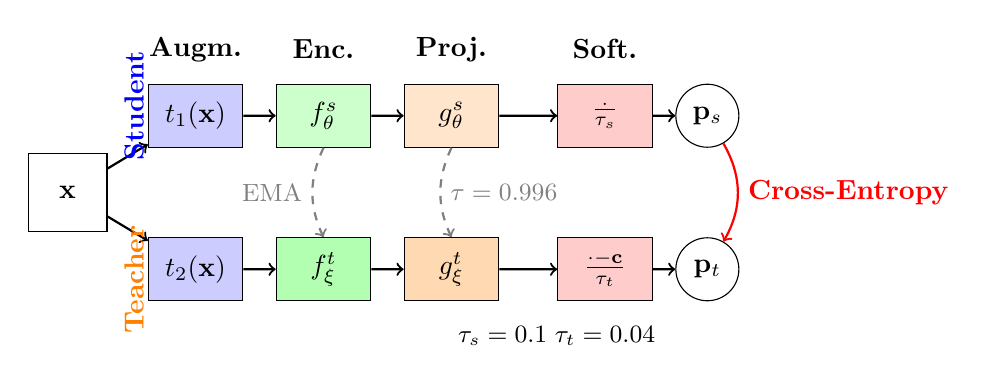
\begin{tikzpicture}[scale=0.65]
% Input image
\node[draw, rectangle, minimum width=1.0cm, minimum height=1.0cm] (input) at (0,0) {$\mathbf{x}$};

% Augmentations
\node[draw, rectangle, fill=blue!20, minimum width=1.2cm, minimum height=0.8cm] (aug1) at (2.5,1.5) {$t_1(\mathbf{x})$};
\node[draw, rectangle, fill=blue!20, minimum width=1.2cm, minimum height=0.8cm] (aug2) at (2.5,-1.5) {$t_2(\mathbf{x})$};

% Student network (top path)
\node[draw, rectangle, fill=green!20, minimum width=1.2cm, minimum height=0.8cm] (enc_student) at (5.0,1.5) {$f_\theta^s$};
\node[draw, rectangle, fill=orange!20, minimum width=1.2cm, minimum height=0.8cm] (proj_student) at (7.5,1.5) {$g_\theta^s$};

% Teacher network (bottom path)  
\node[draw, rectangle, fill=green!30, minimum width=1.2cm, minimum height=0.8cm] (enc_teacher) at (5.0,-1.5) {$f_\xi^t$};
\node[draw, rectangle, fill=orange!30, minimum width=1.2cm, minimum height=0.8cm] (proj_teacher) at (7.5,-1.5) {$g_\xi^t$};

% Temperature (student)
\node[draw, rectangle, fill=red!20, minimum width=1.2cm, minimum height=0.8cm] (temp_student) at (10.5,1.5) {$\frac{.}{\tau_s}$};

% Temperature and centering (teacher)
\node[draw, rectangle, fill=red!20, minimum width=1.2cm, minimum height=0.8cm] (temp_center) at (10.5,-1.5) {$\frac{\cdot - \mathbf{c}}{\tau_t}$};

% Outputs
\node[draw, circle, minimum width=0.8cm] (z_student) at (12.5,1.5) {$\mathbf{p}_s$};
\node[draw, circle, minimum width=0.8cm] (z_teacher) at (12.5,-1.5) {$\mathbf{p}_t$};

% Arrows
\draw[->, thick] (input) -- (aug1);
\draw[->, thick] (input) -- (aug2);
\draw[->, thick] (aug1) -- (enc_student);
\draw[->, thick] (enc_student) -- (proj_student);
\draw[->, thick] (proj_student) -- (temp_student);
\draw[->, thick] (temp_student) -- (z_student);

\draw[->, thick] (aug2) -- (enc_teacher);
\draw[->, thick] (enc_teacher) -- (proj_teacher);
\draw[->, thick] (proj_teacher) -- (temp_center);
\draw[->, thick] (temp_center) -- (z_teacher);

% Loss connection
\draw[->, thick, red, bend left=30] (z_student) to node[midway, right] {\textcolor{red}{\textbf{Cross-Entropy}}} (z_teacher);

% Labels
\node at (2.5, 2.8) {\textbf{Augm.}};
\node at (5.0, 2.8) {\textbf{Enc.}};
\node at (7.5, 2.8) {\textbf{Proj.}};
\node at (10.5, 2.8) {\textbf{Soft.}};

\node at (1.3, 1.7) [rotate=90] {\textcolor{blue}{\textbf{Student}}};
\node at (1.3, -1.7) [rotate=90] {\textcolor{orange}{\textbf{Teacher}}};

% EMA update arrows
\draw[->, dashed, thick, gray] (enc_student.south) to[bend right=25] node[midway, left] {\small EMA} (enc_teacher.north);
\draw[->, dashed, thick, gray] (proj_student.south) to[bend right=25] node[midway, right] {\small $\tau = 0.996$} (proj_teacher.north);

% Temperature labels
\node at (8.5, -2.8) {\small $\tau_s = 0.1$};
\node at (10.5, -2.8) {\small $\tau_t = 0.04$};
\end{tikzpicture}
\end{center}
\vspace{0.5cm}
\alert{Encorder and Projector with the same architecture (required for EMA updates).}

\end{frame}

\begin{frame}{DINO: Symmetric network design}
\textbf{Student network (trainable):}
$$\mathbf{p}_s = \text{softmax}\left(\frac{g_\theta^s(f_\theta^s(\mathbf{x}_1))}{\tau_s}\right)$$
\begin{itemize}
\item \textbf{Encoder:} $f_\theta^s$ - extracts features.
\item \textbf{Projector:} $g_\theta^s$ - maps to representation space.  
\item \textbf{Temperature:} $\tau_s = 0.1$ - controls sharpness.
\end{itemize}

\textbf{Teacher network (EMA updated):}
$$\mathbf{p}_t = \text{softmax}\left(\frac{g_\xi^t(f_\xi^t(\mathbf{x}_2)) - \mathbf{c}}{\tau_t}\right)$$
\begin{itemize}
\item \textbf{Encoder:} $f_\xi^t$ - same architecture as student.
\item \textbf{Projector:} $g_\xi^t$ - same architecture as student.
\item \textbf{Centering:} $\mathbf{c}$ - prevents collapse.
\item \textbf{Temperature:} $\tau_t = 0.04$ - sharper than student.
\end{itemize}

\end{frame}

\begin{frame}{DINO: Implementation for MNIST}
  \textbf{Student encoder:} 
  \vspace{0.3cm}
  \begin{itemize}
  \item Conv2d(1→32) + BatchNorm + ReLU + MaxPool
  \vspace{0.3cm}
  \item Conv2d(32→64) + BatchNorm + ReLU + MaxPool  
  \vspace{0.3cm}
  \item Feature dimension: 256
\end{itemize}

\vspace{0.5cm}

\textbf{Student projection head:}
  \vspace{0.3cm}
\begin{itemize}
\item MLP(256 → 512 → 512 → 256) + BatchNorm + GELU
  \vspace{0.3cm}
\item Output dimension: 256 (for softmax)
\end{itemize}

\vspace{0.5cm}

\textbf{Teacher network:}
  \vspace{0.3cm}
\begin{itemize}
\item \alert{Identical architecture} to student (encoder + projector).
\vspace{0.3cm}
\item \alert{No gradients} - updated only via EMA.
\end{itemize}
\end{frame}

\begin{frame}{DINO: EMA update mechanism}
\textbf{Exponential Moving Average for entire network:}
Teacher parameters updated as:
$$\xi \leftarrow \tau \xi + (1 - \tau) \theta$$
where $\tau \in [0.996, 0.999]$ is the momentum coefficient.

\vspace{0.3cm}

\textbf{Both encoder and projector updated:}
\begin{align*}
f_\xi^t &\leftarrow \tau f_\xi^t + (1-\tau) f_\theta^s \\
g_\xi^t &\leftarrow \tau g_\xi^t + (1-\tau) g_\theta^s
\end{align*}

\vspace{0.3cm}

Implementation details:
\begin{itemize}
\item \textbf{Initialization:} $\xi_0 = \theta_0$ (teacher = student at start).
\vspace{0.3cm}
\item \textbf{Momentum schedule:} $\tau$ increases from 0.996 to 0.999 during training.
\vspace{0.3cm}
\item \textbf{Update frequency:} Every training step (after student gradient update).
\end{itemize}
\end{frame}

\begin{frame}{DINO: Loss function}
\textbf{Cross-entropy loss with centering:}
For augmented pair $(\mathbf{x}_1, \mathbf{x}_2)$,
\begin{align*}
\mathcal{L}_{DINO} = \frac{1}{2}\left[H(\mathbf{P}_t^{(2)}, \mathbf{P}_s^{(1)}) + H(\mathbf{P}_t^{(1)}, \mathbf{P}_s^{(2)})\right]
\end{align*}
  \vspace{0.3cm}
where $H(\mathbf{P}, \mathbf{Q}) = -\sum_k P_k \log Q_k$ is the cross-entropy between distributions $\mathbf{P}$ and $\mathbf{Q}$.
  \vspace{0.3cm}
\begin{itemize}
\item $\mathbf{P}_s^{(1)} = \text{softmax}\left(\frac{g_\theta^s(f_\theta^s(\mathbf{x}_1))}{\tau_s}\right)$ - student distribution for view 1.
  \vspace{0.3cm}
\item $\mathbf{P}_t^{(2)} = \text{softmax}\left(\frac{g_\xi^t(f_\xi^t(\mathbf{x}_2)) - \mathbf{c}}{\tau_t}\right)$ - teacher distribution for view 2.
  \vspace{0.3cm}
\item \textbf{Centering:} $\mathbf{c} \leftarrow 0.9 \mathbf{c} + 0.1 \frac{1}{B}\sum_{b=1}^B g_\xi^t(f_\theta^t(\mathbf{x}_b))$, where $\mathbf{x}_b$ is a batch image and $c$ starts at $0$. 
\end{itemize}

\alert{Intuition: Student distribution should match teacher distribution for different views (code5-dino\_unsupfeatlearn.py).}

\end{frame}

\begin{frame}{Comparison among representations using projections}
  \begin{center}
    \begin{tabular}{ccc}
      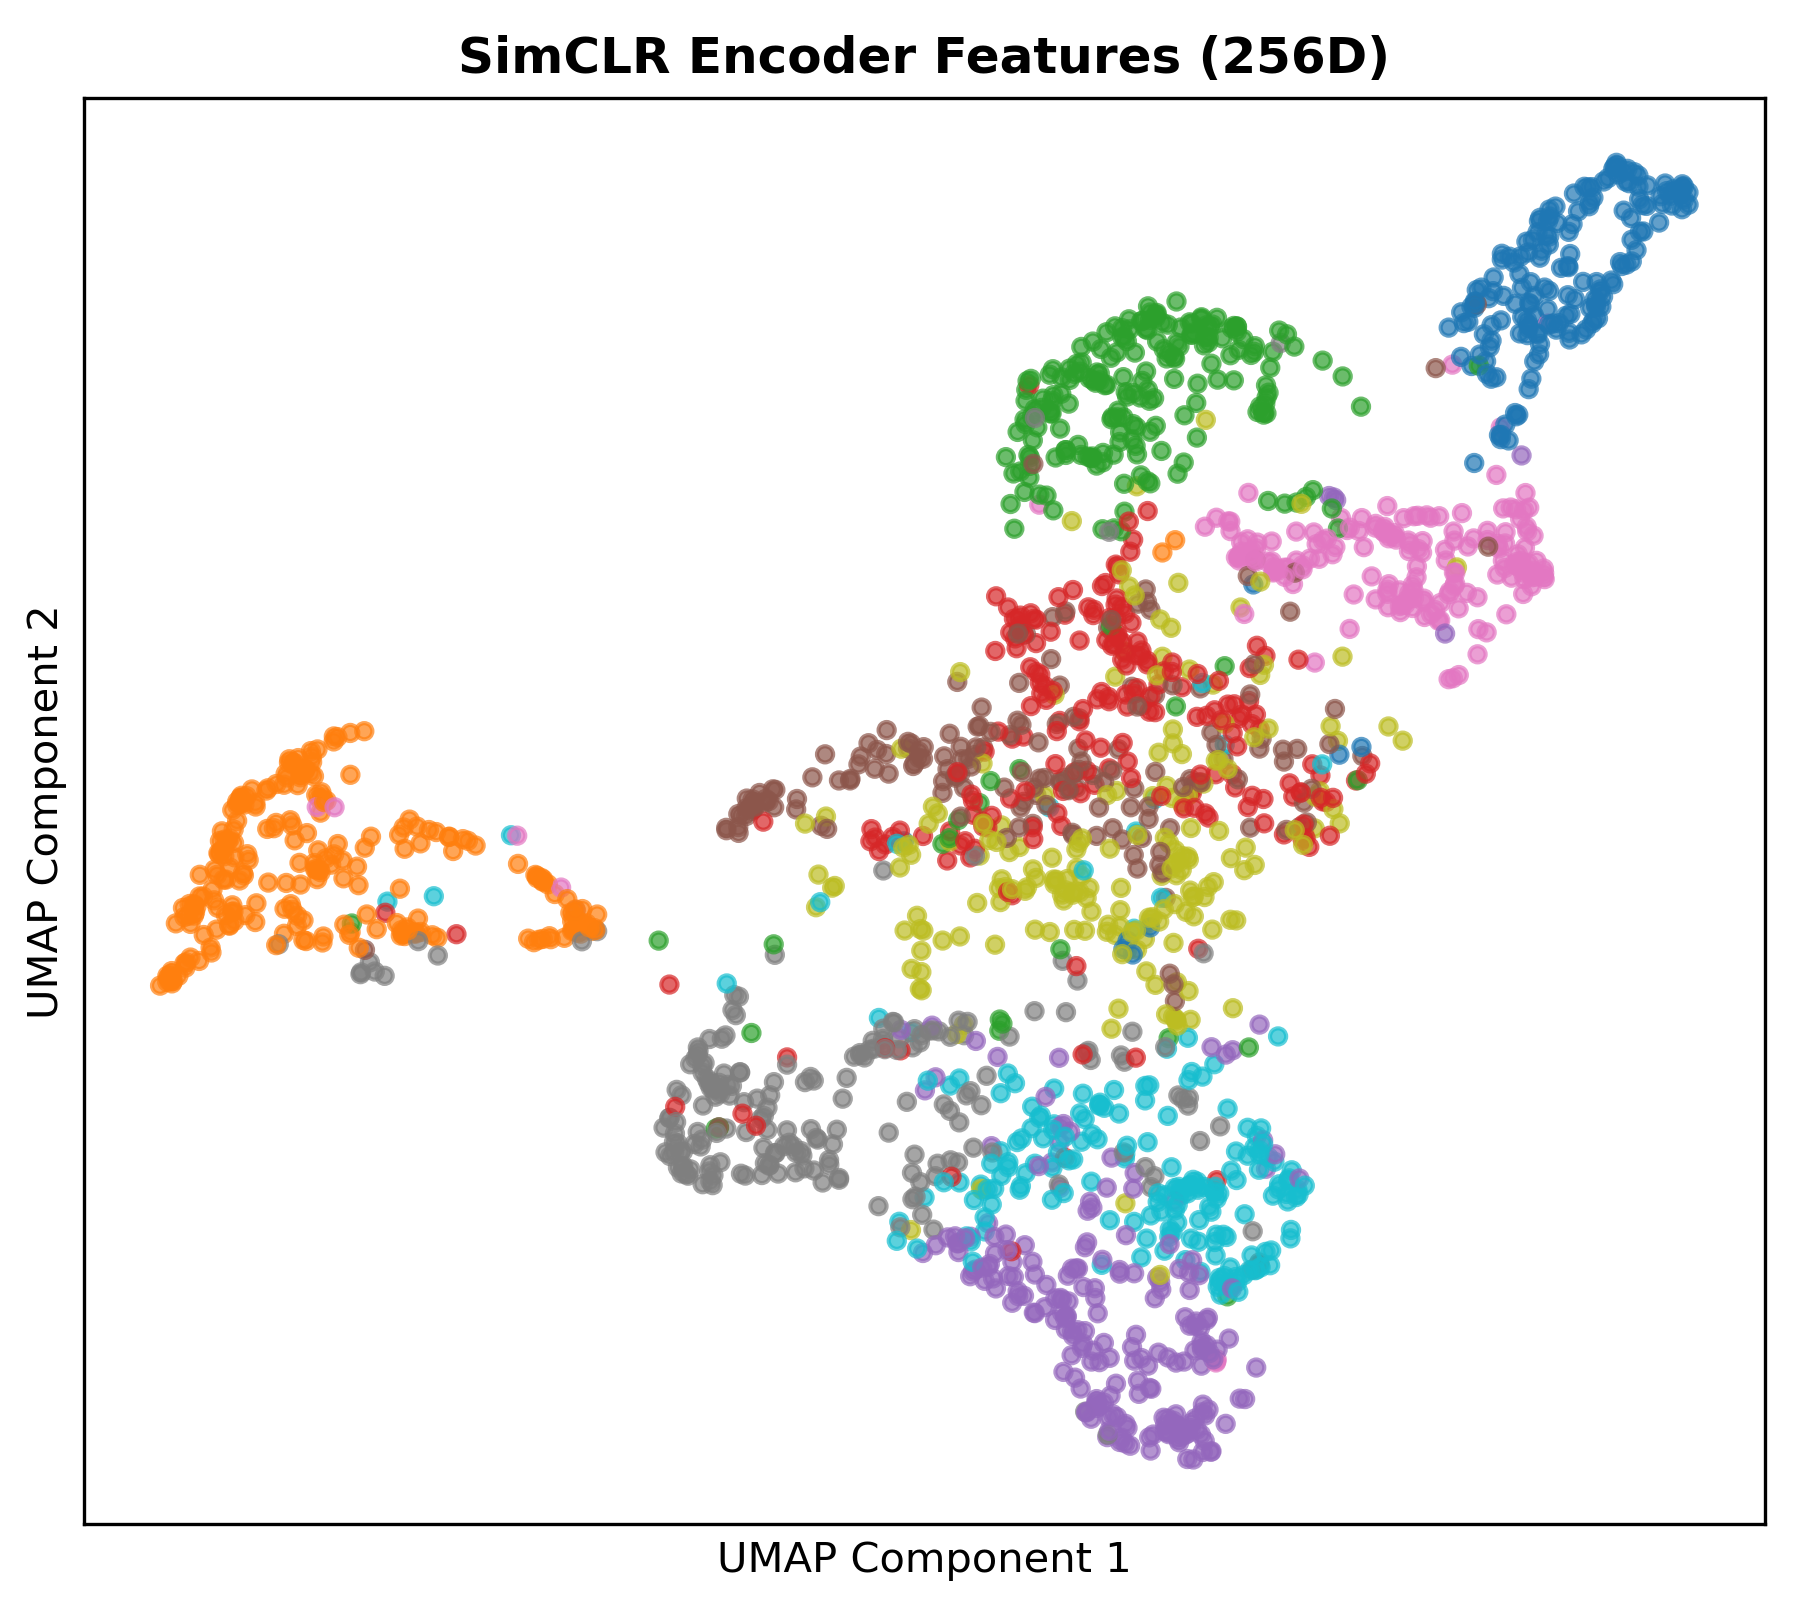
\includegraphics[scale=0.2]{./figs/simclr_umap_projection.png}&
      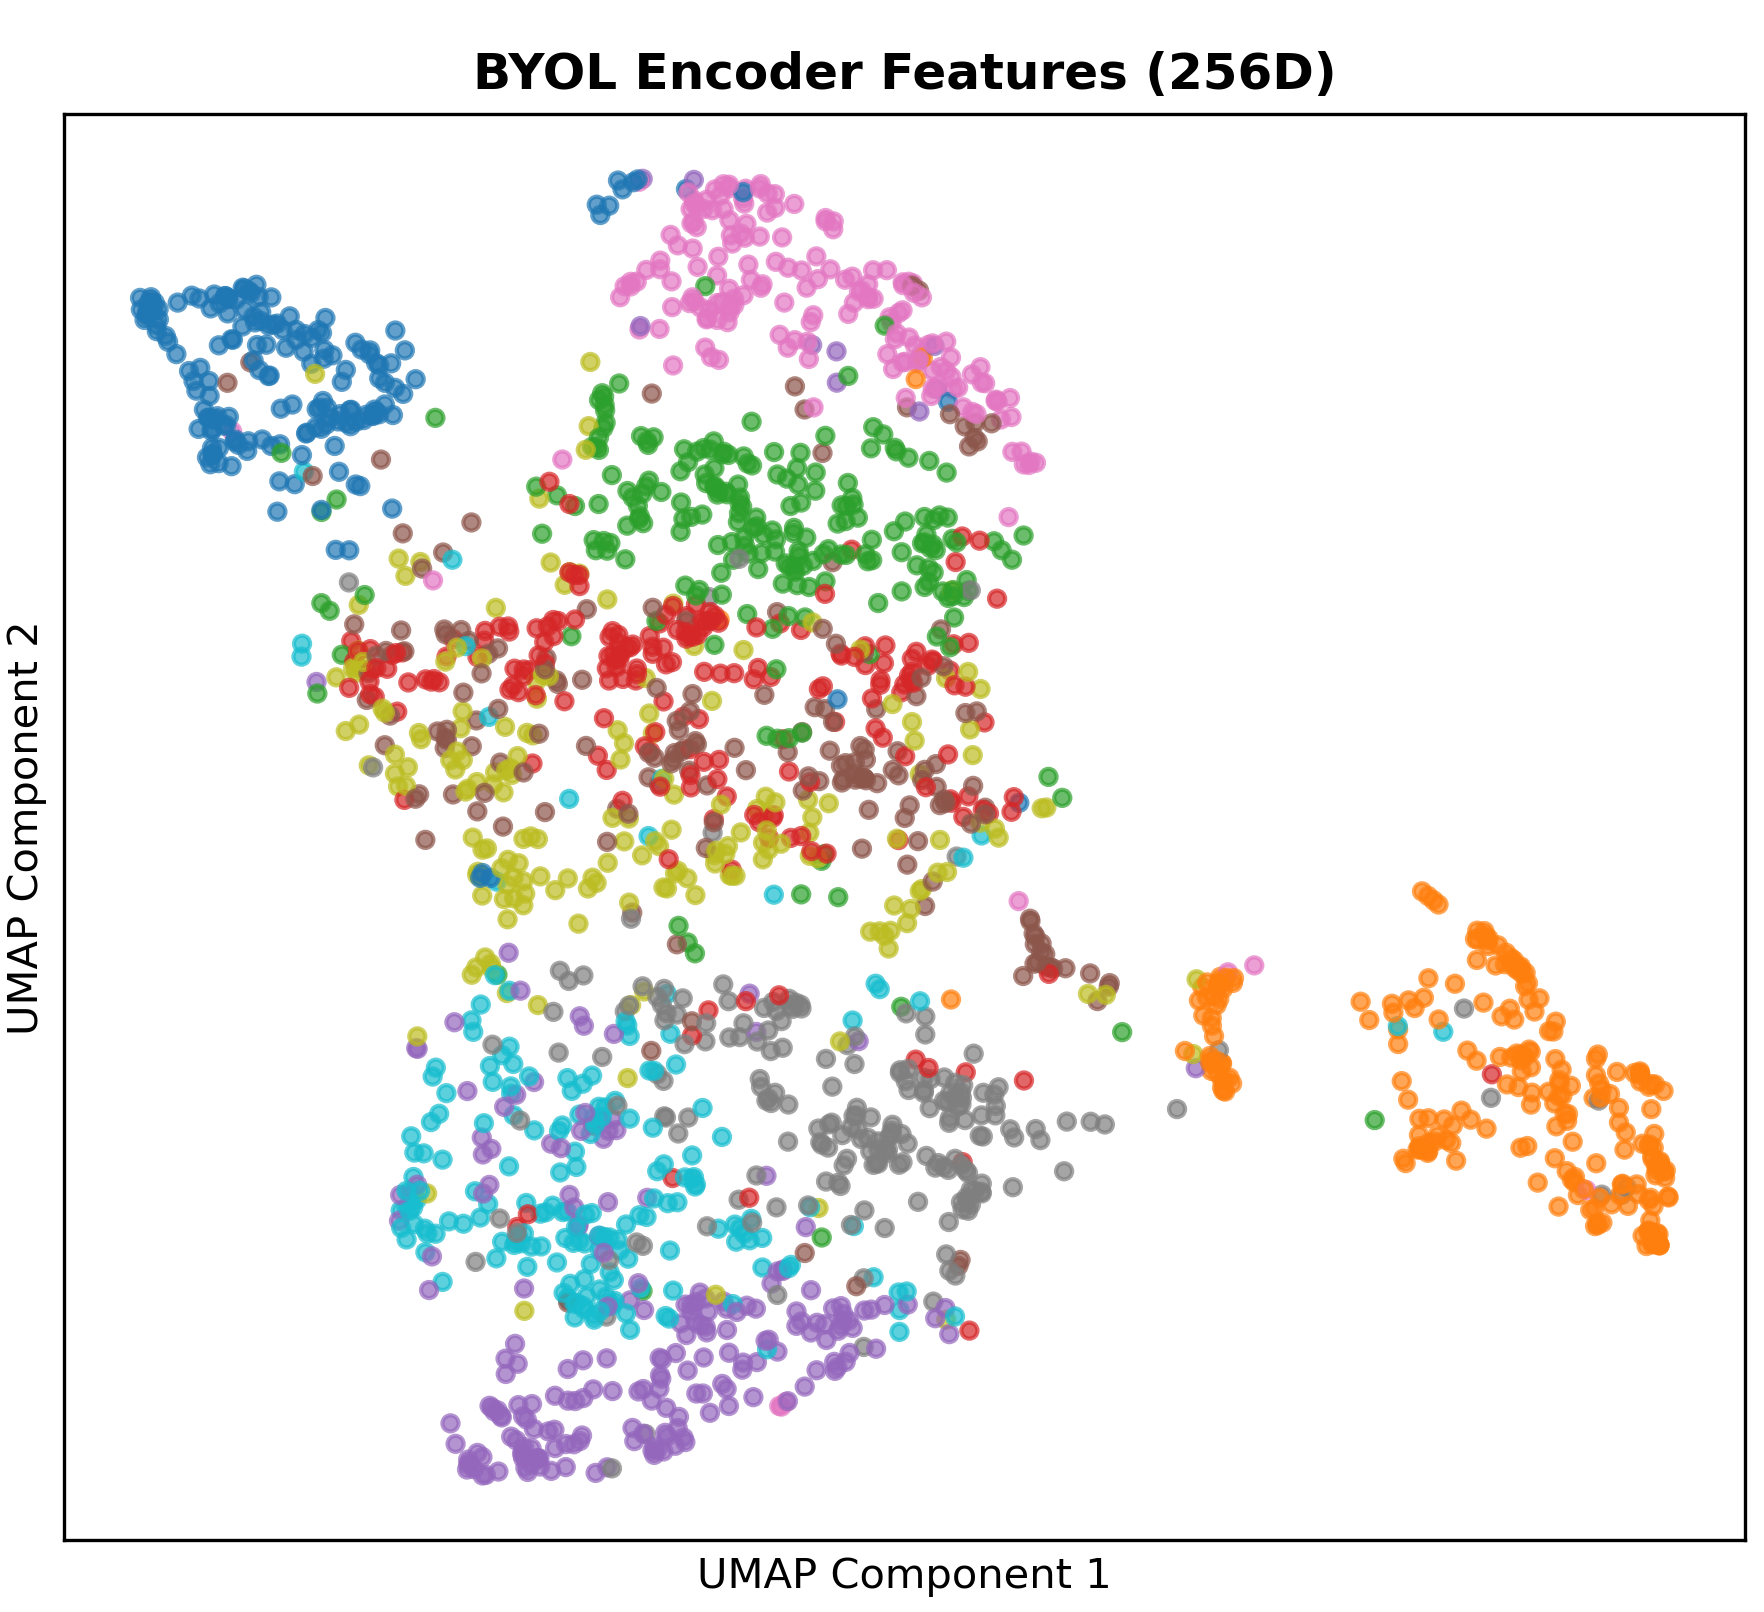
\includegraphics[scale=0.2]{./figs/byol_umap_projection.png}&
      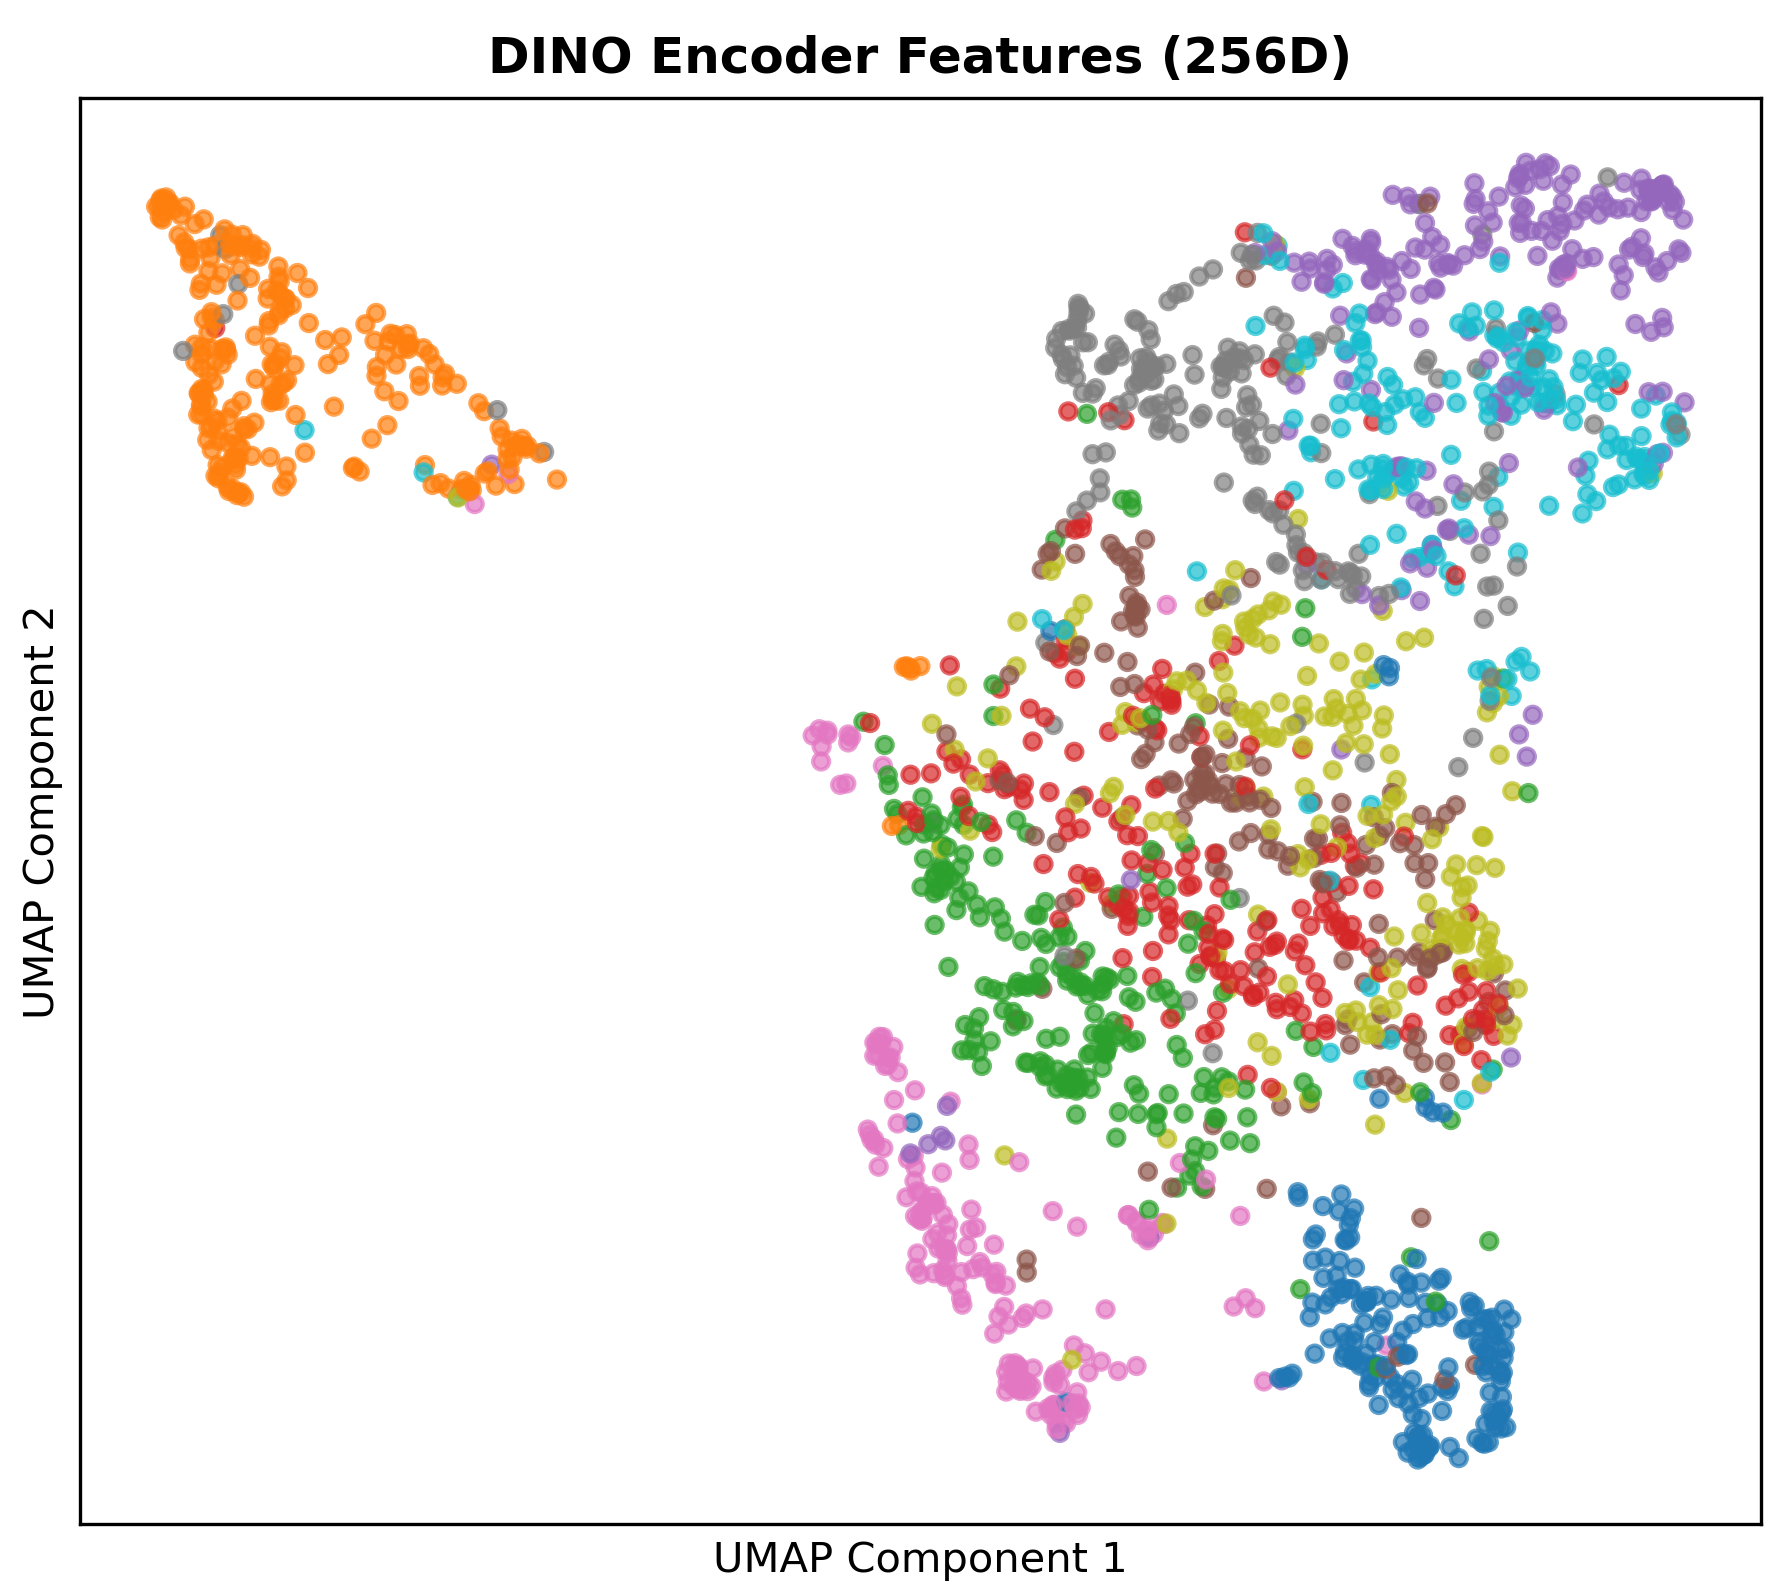
\includegraphics[scale=0.2]{./figs/dino_umap_projection.png}
    \end{tabular}
  \end{center}
Comparison among representations using projections may be misleading;
it is better to evaluate them on a target task.
  
\end{frame}

\begin{frame}{DINO: Multi-crop strategy (Advanced)}
\textbf{True DINO innovation:} Asymmetric multi-crop processing

\vspace{0.2cm}

\textbf{Student receives local crops:}
\begin{itemize}
\item 6-8 small crops (96×96 patches) 
\item Learns from \alert{partial information}
\item Forced to understand global context from local details
\end{itemize}

\vspace{0.2cm}

\textbf{Teacher receives global crops:}
\begin{itemize}
\item 2 large crops (224×224 views)
\item Provides \alert{global semantic context}  
\item Full image understanding
\end{itemize}

\vspace{0.2cm}

\textbf{Loss:} Student (local) → Teacher (global)
$$\mathcal{L} = \sum_{\text{local}} \sum_{\text{global}} \text{CrossEntropy}(\text{student}_{\text{local}}, \text{teacher}_{\text{global}})$$

\alert{This local-to-global learning is DINO's key advantage for natural images! }
\end{frame}

\begin{frame}{DINO: Multicrop examples}

  \begin{center}
\includegraphics[scale=0.17]{./figs/dino_multicrop_examples.png}
  \end{center}

  See code6-dino\_multicrop\_unsupfeatlearn.py.
\end{frame}

\begin{frame}{DINO: Final data representation}

  \begin{center}
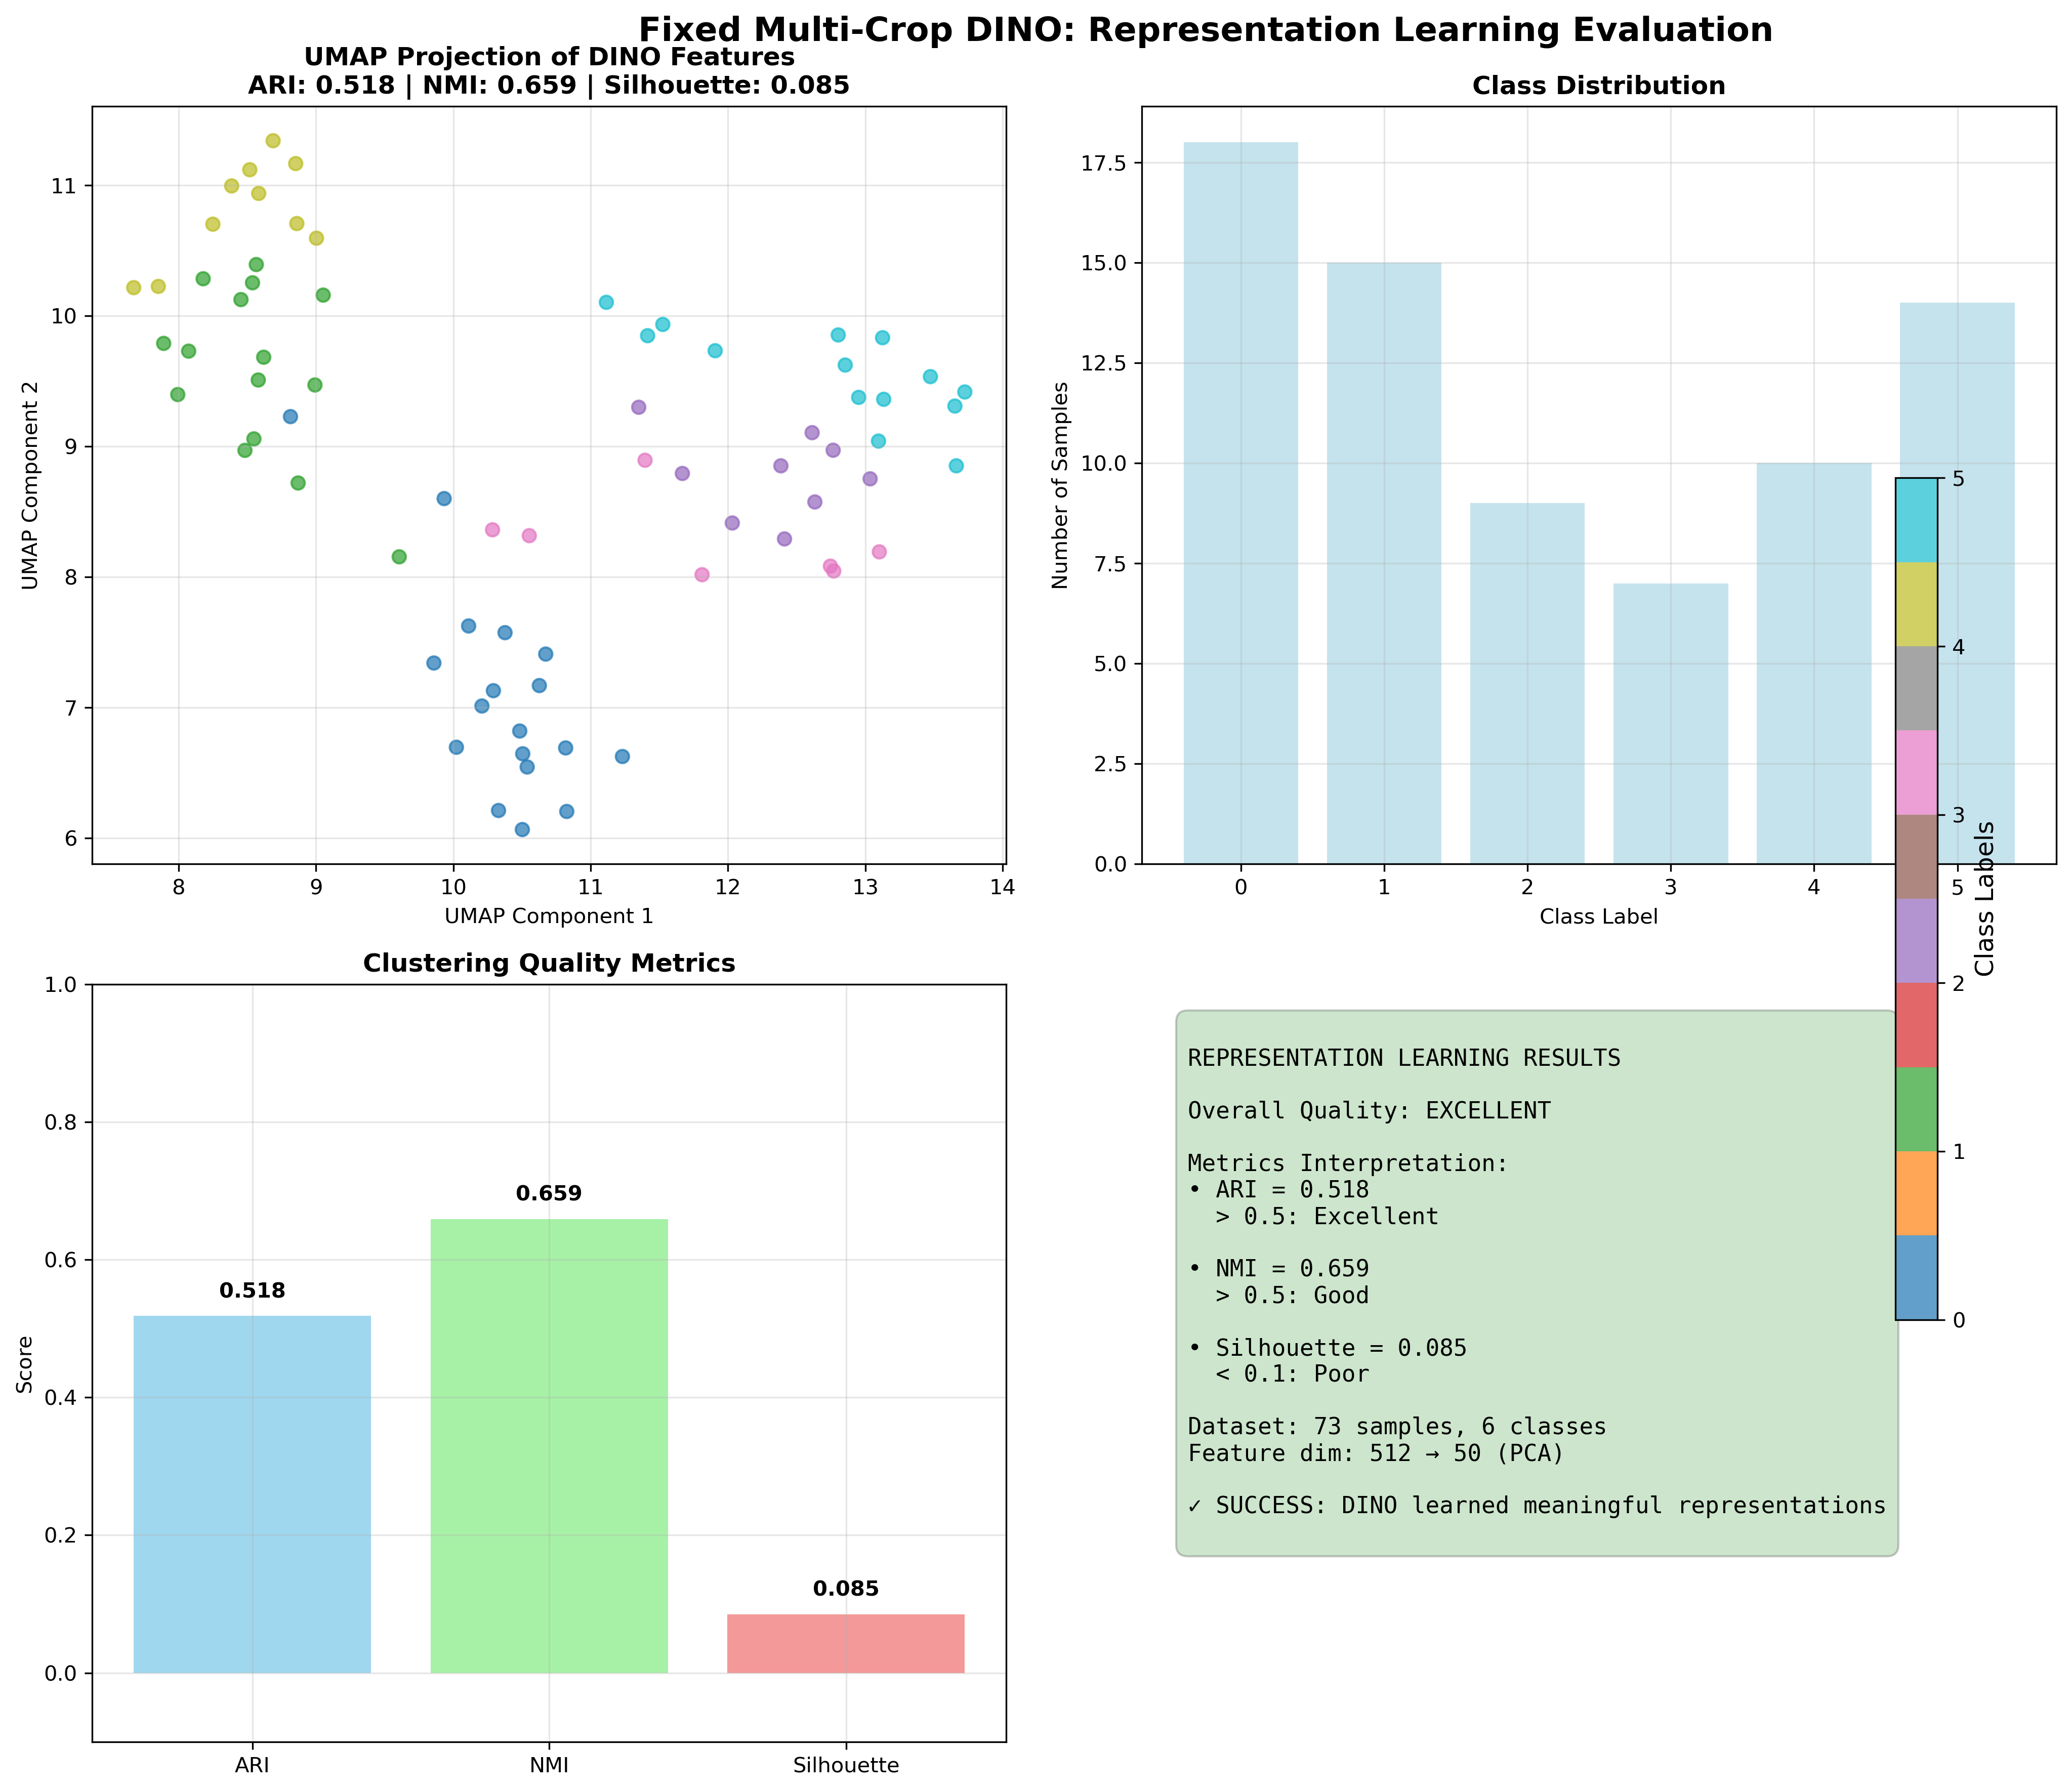
\includegraphics[scale=0.25]{./figs/dino_multicrop_representations.png}
  \end{center}

\end{frame}

\begin{frame}{Why DINO works?}
Without negatives, why does the model not collapse to trivial representations?
   \vspace{0.2cm}
\begin{enumerate}
\item \textbf{Centering mechanism:}
  \vspace{0.2cm}
  \begin{itemize}
  \item Prevents teacher from outputting uniform distributions.
  \item Forces teacher to maintain meaningful output diversity.
  \end{itemize}
  \vspace{0.2cm}   
\item \textbf{Temperature scaling:} Different $\tau_s$ and $\tau_t$
  \vspace{0.2cm}
  \begin{itemize}
  \item Teacher outputs ($\tau_t = 0.04$) are sharper than student ($\tau_s = 0.1$).
  \item Creates informative, peaked target distributions.
  \end{itemize}
  \vspace{0.2cm}
\item \textbf{EMA updates:} Teacher evolves slowly
  \vspace{0.3cm}
  \begin{itemize}
  \item Provides stable targets that gradually improve.
  \item Student cannot immediately "game" the teacher.
  \end{itemize}
\end{enumerate}
\vspace{0.2cm}
\alert{Centering + temperature scaling + EMA = stable self-distillation!}
\end{frame}

\begin{frame}{DINO: Why better than BYOL?}
\textbf{Theoretical advantages:}
\begin{itemize}
\item \textbf{Probabilistic targets:} Cross-entropy loss more principled than MSE.
\item \textbf{No predictor asymmetry:} Softmax is cleaner.
\item \textbf{Multi-crop capability:} Local-to-global learning impossible in BYOL.
\item \textbf{Better collapse prevention:} Centering more reliable than predictor asymmetry.
\end{itemize}

\vspace{0.2cm}

\textbf{Empirical benefits:}
\begin{itemize}
\item \textbf{Better downstream performance:} Especially on dense prediction tasks.
\item \textbf{More stable training:} Less sensitive to hyperparameters.
\item \textbf{Richer representations:} Self-distillation creates more informative features.
\end{itemize}
\vspace{0.2cm}
\alert{DINO represents the evolution from contrastive (SimCLR) → asymmetric (BYOL) → self-distillation approaches.}
\end{frame}

\begin{frame}{References}
  \begin{enumerate}
  \item Noroozi et al. Boosting Self-Supervised Learning via
    Knowledge Transfer,
    \url{https://openaccess.thecvf.com/content_cvpr_2018/papers/Noroozi_Boosting_Self-Supervised_Learning_CVPR_2018_paper.pdf}.
  \item Doersch et al. Unsupervised Visual Representation Learning by Context Prediction, \url{https://arxiv.org/pdf/1505.05192}.
  \item Chen et al. A simple framework for contrastive learning of
    visual representations. ICML 2020.
  \item Grill et al. Bootstrap your own latent: A new approach to
    self-supervised learning. NeurIPS 2020.
  \item Caron et al. Emerging properties in self-supervised vision
    transformers. ICCV 2021.
  \item He et al. Masked autoencoders are scalable vision
    learners. CVPR 2022.
  \end{enumerate}
\end{frame}



\end{document}
